\documentclass{standalone}
\usepackage{tikz}
\usetikzlibrary{matrix,arrows,decorations.pathmorphing,decorations.pathreplacing,calc,positioning}
\usepackage{xcolor}
% all other packages and stuff you need for the picture
\newcommand{\myunit}{0.65 cm}
\newcommand{\myraise}{3pt}
\tikzset{
    lpltsty/.style={decorate, decoration = {brace,mirror,raise=3pt,amplitude=5pt}},
    namesty/.style={pos=0.5,below=7pt},
    scalarsty/.style={draw,fill=white,rectangle,minimum size=\myunit,anchor=center},
    indexsty/.style={fill,fill=white,rectangle,minimum width=\myunit,anchor=center},
    touchsty/.style={fill,fill=red,rectangle,minimum size=\myunit},
    ycsty/.style={fill,fill=yellow,rectangle,minimum size=\myunit},
    brcsty/.style={fill,fill=brown,rectangle,minimum size=\myunit},
    blcsty/.style={fill,fill=cyan!20,rectangle,minimum size=\myunit},
    becsty/.style={fill,fill=beige,rectangle,minimum size=\myunit},
    ocsty/.style={fill,fill=orange,rectangle,minimum size=\myunit},
    whclsty/.style={fill,fill=white,rectangle,minimum size=\myunit},
    zcsty/.style={fill,fill=white,rectangle,minimum size=\myunit,text=zerogray},
    nzsty/.style={fill,fill=black,rectangle,minimum size=\myunit,text=white},
    rcsty/.style={fill,fill=purple,rectangle,minimum size=\myunit},
    pcsty/.style={fill,fill=pink,rectangle,minimum size=\myunit},
    lcsty/.style={fill,fill=blue,rectangle,minimum size=\myunit},
    bcsty/.style={fill,fill=black,rectangle,minimum size=\myunit, text=white},
    hlsty/.style={draw=red},
}


\colorlet{zerogray}{gray!25}
\colorlet{beige}{brown!70}

\newcommand{\ylcl}{|[ycsty]|1}
\newcommand{\recl}{|[rcsty]|2}
\newcommand{\picl}{|[pcsty]|3}
\newcommand{\blcl}{|[blcsty]|1}
\newcommand{\brcl}{|[brcsty]|2}
\newcommand{\becl}{|[becsty]|3}
\newcommand{\orcl}{|[ocsty]|4}
\newcommand{\bkcl}{|[bcsty]|5}
\newcommand{\whcl}{|[whclsty]|0}
\newcommand{\zecl}{|[zcsty]|0}

\newcommand{\formatscale}{0.5}
\newcommand{\matrixscale}{0.69}
\begin{document}

\resizebox{\linewidth}{!}{%
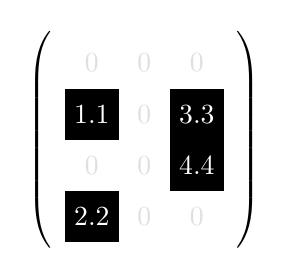
\begin{tikzpicture}[>=latex]
\matrix (A) [matrix of math nodes,
  nodes = {whclsty},
  left delimiter  = (,
  right delimiter = ),
  ampersand replacement=\&] at (0,0)
{
\zecl \& \zecl \& \zecl\\
|[nzsty]|1.1 \& \zecl \& |[nzsty]|3.3 \\
\zecl \& \zecl \& |[nzsty]|4.4\\
|[nzsty]|2.2 \& \zecl \& \zecl\\
};
\end{tikzpicture}%
}
\resizebox{2.0\linewidth}{!}{%
\begin{tikzpicture}[>=latex]

  \matrix (Af) [matrix of math nodes,
    nodes = {whclsty},
    left delimiter  = (,
    right delimiter = ),
    ampersand replacement=\&,
    anchor=north west] at (10.0*\myunit, 0*\myunit)
{
|[fullsty]|\&|[fullsty]|\&|[fullsty]|\\
};
\matrix (Af-1-1f) [matrix of math nodes,
    nodes = {whclsty},
    left delimiter  = (,
    right delimiter = ),
    ampersand replacement=\&,
    anchor=north west] at (6.0*\myunit, 2*\myunit)
{
|[fullsty]|\&|[fullsty]|\&|[fullsty]|\\
};
\node (Af-1-1f-1-1f) [nzsty] at (0*\myunit, 4*\myunit) {11};
\draw (Af-1-1f-1-1.center) -- (Af-1-1f-1-1f.north) node [midway, fill=white] {$i$=1};
\node (Af-1-1f-1-2f) [nzsty] at (1*\myunit, 4*\myunit) {22};
\draw (Af-1-1f-1-2.center) -- (Af-1-1f-1-2f.north) node [midway, fill=white] {$i$=2};
\node (Af-1-1f-1-3f) [nzsty] at (2*\myunit, 4*\myunit) {33};
\draw (Af-1-1f-1-3.center) -- (Af-1-1f-1-3f.north) node [midway, fill=white] {$i$=3};
\draw (Af-1-1.center) -- (Af-1-1f.north) node [midway, fill=white] {$i$=1};
\matrix (Af-1-2f) [matrix of math nodes,
    nodes = {whclsty},
    left delimiter  = (,
    right delimiter = ),
    ampersand replacement=\&,
    anchor=north west] at (12.0*\myunit, 2*\myunit)
{
|[fullsty]|\&|[fullsty]|\&|[fullsty]|\\
};
\node (Af-1-2f-1-1f) [nzsty] at (12*\myunit, 4*\myunit) {44};
\draw (Af-1-2f-1-1.center) -- (Af-1-2f-1-1f.north) node [midway, fill=white] {$i$=1};
\node (Af-1-2f-1-2f) [nzsty] at (13*\myunit, 4*\myunit) {55};
\draw (Af-1-2f-1-2.center) -- (Af-1-2f-1-2f.north) node [midway, fill=white] {$i$=2};
\node (Af-1-2f-1-3f) [nzsty] at (14*\myunit, 4*\myunit) {66};
\draw (Af-1-2f-1-3.center) -- (Af-1-2f-1-3f.north) node [midway, fill=white] {$i$=3};
\draw (Af-1-2.center) -- (Af-1-2f.north) node [midway, fill=white] {$i$=2};
\matrix (Af-1-3f) [matrix of math nodes,
    nodes = {whclsty},
    left delimiter  = (,
    right delimiter = ),
    ampersand replacement=\&,
    anchor=north west] at (12.0*\myunit, 2*\myunit)
{
|[fullsty]|\&|[fullsty]|\&|[fullsty]|\\
};
\node (Af-1-3f-1-1f) [nzsty] at (12*\myunit, 4*\myunit) {77};
\draw (Af-1-3f-1-1.center) -- (Af-1-3f-1-1f.north) node [midway, fill=white] {$i$=1};
\node (Af-1-3f-1-2f) [nzsty] at (13*\myunit, 4*\myunit) {88};
\draw (Af-1-3f-1-2.center) -- (Af-1-3f-1-2f.north) node [midway, fill=white] {$i$=2};
\node (Af-1-3f-1-3f) [nzsty] at (14*\myunit, 4*\myunit) {99};
\draw (Af-1-3f-1-3.center) -- (Af-1-3f-1-3f.north) node [midway, fill=white] {$i$=3};
\draw (Af-1-3.center) -- (Af-1-3f.north) node [midway, fill=white] {$i$=3};

\end{tikzpicture}%
}

\end{document}